% !TEX root = ../report.tex

\chapter{Software}\label{software}

\todo{Bit in here about overall structure and architecture}



\section{ROS}\label{soft/ROS}

\subsection{Design}\label{soft/ROS/design}

\subsection{Implementation}\label{soft/ROS/impl}

\subsection{Testing}\label{soft/ROS/test}



\section{Communication}\label{soft/comms}

\subsection{Design}\label{soft/comms/design}

\subsection{Implementation}\label{soft/comms/impl}

\subsection{Testing}\label{soft/comms/test}




\section{SLAM \& Sensor Fusion}\label{soft/SLAM}

\subsection{Design}\label{soft/SLAM/design}

\subsection{Implementation}\label{soft/SLAM/impl}

\subsection{Testing}\label{soft/SLAM/test}



\section{Computer Vision}\label{soft/cv}
Computer vision is a very cheap and effective way of gaining a high level understanding of the environment. It was used to allow the agents to identify other robots and objectives in in the system. Detecting the other robots was an essential component to allow communication between robots, prevent agents mistakenly mapping other agents,and to recognise when ultrasonic interference would occur. 

\subsection{Design}\label{soft/cv/design}
The first detection system considered was a CNN, as discussed in \ref{litreview/cv/objDet/CNN}.This is a very effective system which has the advantage of 
being able to classify instances of objects that it has not 
seen before. This would be essential if the target objects of 
the robot was not consistent, for instance if it had to find 
people in the search space. This was, however, not essential 
in the scope of this project. The major downside to this 
system would be the time to implement. To construct a CNN for 
this application would require the collection of a large data 
set of images of the robots and goals, as well as the time 
consuming process of tuning the CNN. 

Feature Based Object detection was also considered. As described in Section \ref{litreview/cv/objDet/fb}, thisonly requires a picture to be taken of the object and therefore takes far less time to 
implement than the CNN solution. However, the accuracy and 
consistency are largely dependant on the number of features 
detected, and the algorithm's complexity grows relatively 
quickly. The basic brute force algorithm involves comparing 
every key point in the object image to every key point in the 
frame image, which results in an O($n^2$) complexity (although 
this can be streamlined, for instance if it becomes impossible 
for the distance to be low enough for a pair to be the best 
match part way through the distance calculation, it does not 
need to be finished). The calculations for deciding the best 
outline of the object also become more complicated, as there 
will be a lower true positive to false positive ratio as the 
best matches (which are found first) are more likely to be 
true positives. It was decided that this would be too  
computationally intensive considering the strict constraint of 
using a Raspberry Pi. 

The method used was by far the simplest considered. It identified the other robots and target by their colour. This was only possible as each robot used had a distinct coloured chassis, which lacks scalability, but was considered an acceptable simplification as this was not the focus of the project. 

This works by first converting the images from RGB to Hue-Saturation-Value (HSV) colour space, simplifying the colour detection as the hue of the pixel is determined by a single value instead of the ratio of three values. A colour can then be identified by a range of H values and then a minimum S and V values, which is far more intuitive than checking if it falls into a range of ratios between R, G and B values. 

\subsection{Implementation}\label{soft/cv/impl}
The \textit{vision\_node} works using a ROS spin setup, with a \textit{spin()} function being called at a set frequency until ROS closes. 

A \textit{RobotDetector} object is declared which has the range of HSV values for each robot and the goal, and has a video capture object. It contains a \textit{search()} function which takes a frame as a parameter and returns various details about each robot's presence in the frame. \textit{search()} first calls \textit{get\_colour\_mask()} for each range of colour values. This converts the image to HSV, then makes a frame, \textit{mask}, which is white where the pixel in range and and black for out of range. This is shown in Code Listing \ref{lst:get_colour_mask}. This also shows the handling of cases where the range of colours crosses the zero point (as zero is adjacent to 255 in the hue value).

\begin{lstlisting}[caption={get\_colour\_mask in RobotDetector},label={lst:get_colour_mask} , language=python]

def get_colour_mask(self, frame, lower_hsv_bound, higher_hsv_bound):
        hsv_frame = cv2.cvtColor(frame, cv2.COLOR_BGR2HSV)

        if (lower_hsv_bound[0] > higher_hsv_bound[0]):
            mask1 = cv2.inRange(hsv_frame, np.array([0, lower_hsv_bound[1], lower_hsv_bound[2]]),
                                np.array(higher_hsv_bound))
            mask2 = cv2.inRange(hsv_frame, np.array(lower_hsv_bound),
                                np.array([179, higher_hsv_bound[1], higher_hsv_bound[2]]))
            mask = mask1 | mask2
        else:
            lower = np.array(lower_hsv_bound)
            upper = np.array(higher_hsv_bound)
            mask = cv2.inRange(hsv_frame, lower, upper)

\end{lstlisting}

The function then uses erosion and dilation functions provided by opencv to reduce noise in the mask. 

The contours in the mask are then iterated through to find the biggest, which is assumed to be the object and the centre point and outline of the contour is found. If no contours are bigger than a fixed size (measured in pixels) the object is assumed to not be in the image frame, and the corresponding \textit{obj\_found} variable is set to false. This process is shown in Code Listing \cite{lst:cv_search_loop}.

\begin{lstlisting}[caption={Contour Iteration in search()},label={lst:cv_search_loop} , language=python]
...
for c in contours:
    if cv2.contourArea(c) > max((300, maxsize)):  
        maxsize = cv2.contourArea(c)
        cx, cy = self.get_centre_point(c)
        outline = self.get_outline(c)
        obj_found = True
...
\end{lstlisting}

These parameters are then returned to the \textit{\_tick()} function which was called by \textit{spin()}. This then renders debug info to the frame if it's performing a test, or publishes the detected robot info via a ROS message consisting of a comma separated list of objects detected in the last frame. 

\subsection{Testing}\label{soft/cv/test}
Initial testing of the \textit{vision\_node} was performed on a PC with a USB webcam. The testing was performed by using the position information to render labelled rectangles to a real time stream highlighting the position of the objects. The code for this is shown in Code Listing \ref{lst:draw_rectangles}. 

\begin{lstlisting}[caption={asd},label={lst:draw_rectangles} , language=python]
for i, name in enumerate(names):
    if found[i]:
        #cv2.drawContours(frame, [outline], -1, (0, 255, 0), 2)
        #cv2.circle(frame, (cx, cy), 7, (255, 255, 255), -1)
        x, y, w, h = cv2.boundingRect(outlines[i])
        cv2.rectangle(frame, (x, y), (x + w, y + h), highlight_colours[i], 2)
        cv2.putText(frame, name, (x - 20, y - 20),
                            cv2.FONT_HERSHEY_SIMPLEX, 0.5, highlight_colours[i], 2)
\end{lstlisting}

An example of this running is shown in Figure \ref{fig:cv_screenshot}

\begin{figure}[!ht]
	\centering
	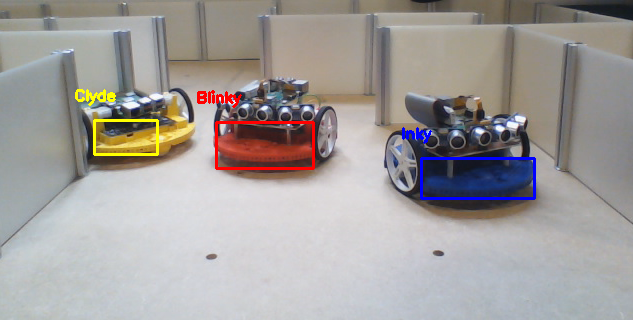
\includegraphics[width=1\textwidth]{ComputerVisionScreenshot.png}
	\caption{Computer Vision PC Test}\label{fig:cv_screenshot}

\end{figure}

The system was then tested on the RPi by monitoring the ROS topic \textit{robots_detected} to test both the integration with the RPi and with ROS. Various detectable objects were moved in and out of the frame and changes in the output were observed. This initially failed as the RPi camera was connected using a CSI port, not a USB port, which OpenCV's VideoCapture function does not support. When running on the RPi, this was replaced with imutil's VideoStream package. After this the test performed as expected, consistently identifying which objects were in frame.  

Functionality was then added to record the feed as to see how the computer vision responded as the robot was traversing the maze, however there were issues with frame rate as it was too computationally intensive for the RPi to perform the recording as well as all the other computation. 

\section{AI \& Control Modules}\label{soft/ai}

\subsection{Design}\label{soft/ai/design}

\subsection{Implementation}\label{soft/ai/impl}

\subsection{Testing}\label{soft/ai/test}